\documentclass[9pt,twocolumn,twoside]{../../styles/osajnl}
\usepackage{fancyvrb}
\journal{i524} 

\title{Introduction to H2O}

\author[1]{Sushmita Sivaprasad}


\affil[1]{School of Informatics and Computing, Bloomington, IN 47408, U.S.A.}


\affil[*]{ sushsiva@umail.iu.edu}

\dates{\today}

\ociscodes{machine learning, data mining,predictive analytics,cloud}

% replace this with your url in github/gitlab
\doi{\url{https://github.com/SushmitaSivaprasad/sp17-i524/tree/master/paper1/S17-IR-2038/report.pdf}}


\begin{abstract}
  
Machine learning and data mining have been used in many data driven
industries. H2O is a platform using for performing machine learning
and predictive analytics for large scale data using cloud. When the
data that is generated is large scale and is in terrabytes, H2O serves
a very important purpose of being able to accurately predict using
different algorithms and also using different programming languages
through APIs. This paper gives an introduction to H2O, how this
platform has impacted various industries across several domains with
improved accuracy and reduced processing time. Different use cases of
the H2O platform has been explained as well.
  
\end{abstract}

\setboolean{displaycopyright}{true}

\begin{document}

\maketitle

\section{Introduction}

H2O is an open source platform that is used to create machine learning
and predictive analytics models on big datasets. It is mainly written
in Javascript but have APIs for R , Python, Excel, Tableau and
Flow\cite{www-h2o-webpage}. The main algorithms implemented on the
datasets are deep learning, gradient boosting , generalized linear
model, distributed random forest and k-means. The algorithms
implemented on the big datasets is read in a parallel manner and is
then distributed and stored in memory in a compressed column
format. H2O also has an inbuilt intelligence to detect and support the
process of obtaining data and importing them for immediate use or
storing in a database which can be obtained from various sources in
different formats\cite{www-h2o-webpage}.


\section{How does H2O work?}

H2O is used on large dataset , usually in the range of terrabytes due
to it's speed in processing the data. A company might have their
dataset stored on big data systems such as Hadoop. On analyzing a data
we usually choose a smaller sample dataset rather than the entire
dataset to build a model due to the large processing time
involved. H2O has the advantage of being able to use the entire
dataset to run the algorithm on a larger dataset, the more the data we
are able to analyse better the predictions would
be\cite{www-h2oyoutubevideo}. Suppose a business is trying to
understand the best product placement for optimal customer enagement,
the model would be created based on the dataset formed collecting
information about the interactions of the customers on the
website. H2O is used to model the data with multiple algorithms using
more than one machine at the same time, this way we don’t have to
sample the data\cite{www-h2oyoutubevideo}. H2O is also used to score
hundreds of models in nano seconds to check which algorithm works
better for that dataset.


\section{Requirements}

\subsection{Operating Systems}

It works on the following operating systems 
\newline Windows 7 or later
\newline OSX 10.9 or later
\newline Ubuntu 12.04
\newline RHEL/CentOS6 or later\cite{www-h2o-requirements}

\subsection{Languages}

 Java 7 or later
\newline Scala 2.10 or later
\newline R version 3 or later
\newline Python 2.7x or 3.5x\cite{www-h2o-requirements}
 
\subsection{Browser}

 Chrome
\newline Safari
\newline Internet Explorer
\newline Firefox\cite{www-h2o-requirements}

\subsection{ Hadoop}
 Optional Cloudera CDH 5.2 or later
\newline MapR 3.1.1 or later
\newline Hortonworks HDP 2.1 or later\cite{www-h2o-requirements}


\subsection{Supported File Formats}

H2O supports the following file types
\newline CSV files
\newline ORC
\newline ARFF
\newline XLSX
\newline XLS
\newline Avro
\newline Parquet\cite{www-h2o-requirements}

More information can be obtained from the documentation provided on
the H2O website\cite{www-h2o-requirements}.

\section{Architecture}

The H2O architecture consists of different components which combine
together to form the H2O software stack.\newline We can divide the H2O
architecture into 3 different components, top section includes all the
REST API clients, middle includes the Network Cloud and the bottom
section contains the different components that run within an H2O JVM
process\cite{www-h2o-architecture}. The top section contains the
programming languages that can be used on the big dataset here. The
REST API clients communicate with the H2O with the help of a socket
connection\cite{www-h2o-architecture}. The Network cloud consists of
the different inbuilt algorithms to create the necessary model on the
data, this can also contain a customized customer algorithm to analyze
the required dataset and produce the desired outputs.


\subsection{REST API Clients}

\begin{itemize}
  \item Javascript: The H2O Web UI is written in the javascript language.
\item R: Using the H2O R package known as 'library(h2o)' the users can write their own R functions.
\item Python: The Python scripts must use the REST API directly as a library for this has not been extablished yet but would be released in the future.
\item Excel: H2O provides an H2O worksheet for Microsoft Excel, which allows us to import the big datasets and run the algorithms.
\item Tableau: The users of H2O may pull results from H2O to create visualizations in Tableau.
\item Flow: This is a notebook style WEB UI for H2O\cite{www-h2o-architecture}.
\end{itemize}

\subsection{JVM Components}

The H2O cloud can consists of two or more nodes
which can contain a single JVM process. Each JVM process consists of
language, algorithm and infrastructure (manages the resources
management such as memory and CPU)\cite{www-h2o-architecture}.

\begin{figure}[htbp]
\centering
\fbox{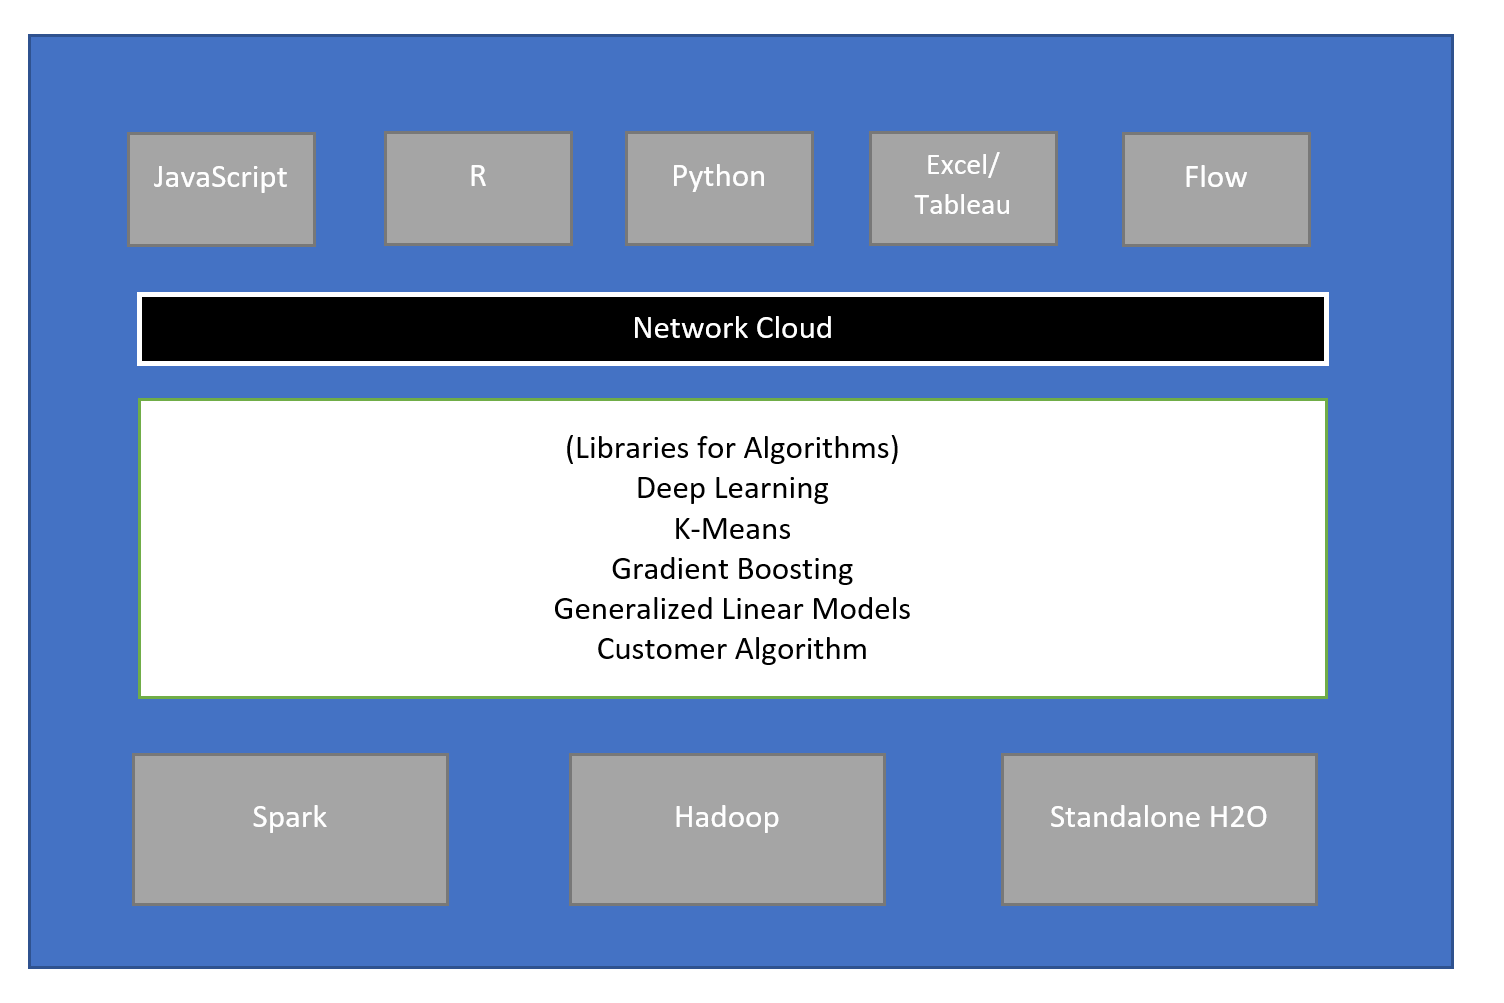
\includegraphics[width=\linewidth]{images/Architecture(1)}}
\caption{H2O Architecture\cite{www-h2o-architecture}}
\label{ fig:Architecture of H2O}
\end{figure}


\section {Used Cases}


\subsection {CapitalOne}

CapitalOne, a fortune 500 bank with 960 banks and 2000 ATMs
accumulates terrabytes of information in real time on customer
information and financial processing. H2O software was implemented in their systems and  was used to reduce the
process time of the algorithm implementations over the large data sets\cite{www-h2o-capitalone}. Different algorithms can be applied to find which one
works best due to reduction in time consumed in processing these large
datasets. A large number of hard and soft metrics were evaluated as
well using machine learning frameworks\cite{www-h2o-capitalone}.Using H2O they were able to process data received from credit cards the moment they were swiped, using this information new offerings were marketed to the customer based on their spending habits.


\subsection {MarketShare}

The company MarketShare have implemented H2O to optimize budgeting for
marketing. Since marketing approaches are data driven features ,
predictive analytics under H2O was used to give a comparison on how
the current state of the marketing budget is and how much is the
predicted revenue\cite{www-h2o-marketshare}. Using H2O, solutions were generated as to what are
the changes that can be made to improve the current projection and
what an improved projection will look like. MarketShare was able to go on the cloud and use as much
machines as required and get desired outputs on the large
datasets. They use 25 machines for all of their clients to process the
data and were able to expand the scalability of the dataset.If their
datasize increases by x amount then they would add y more machines to
solve the problem\cite{www-h2o-marketshare}. Scaling across lot of nodes is critical to their
business as the company deals with digital log data and irrespective
of the complexity of the modelling and the huge size of the data\cite{www-h2o-marketshare}. MarketShare was able to generate marketing plans and what-if cases based on the information from their customers using different predictive analytics models.

\section {Relevant Resources}

H2O has an open source platform and hence has a community for support.
\begin{itemize}
\item Step by step instructions with documentation and videos have
   been provided for installation and to understand the work flow of
   H2O\cite{www-h2o-webpage}.
\item Free online training videos are provided on the main webpage
  \cite{www-h2o-learn}.
\item H2O documentation is available on their website
  \cite{www-h2o-webpage}.
\item h2ostream is an open source google group where H2O users can
    post questions and get answers.
\item They have built an online community at\cite{www-h2o-community}
  which is a discussion platform.
\item They also conduct conferences around the year in United States
    for users to interact among one another and update new releases
    and happenings in the big data community\cite{www-h2o-meetups}.
\end{itemize}


\section{Conclusion}

Being an open source platform it gives user the flexibility to solve
the problems. It is easy to set up and has a smooth installation and
usage feature due to its interface with familiar programming
environments using APIs\cite{www-h2o-why}. Models can also be
inspected during training.It can process any format of file , it can
even connect to data from HDFS, S3 ,SQL and NoSQL data
sources\cite{www-h2o-why}.It has a large scalability hence allowing
large datasets to be analyzed by using multiple machines. It also
conducts a real time data scoring for accurate
predictions\cite{www-h2o-why}.

\section{Acknowledgement}

A very special thanks to Professor Gregor von Laszewski and the
teaching assistants Miao Zhang and Dimitar Nikolov for all the support
and guidance in getting this paper done and resolving all the
technical issues faced. The paper is written during the spring 2017
semester course {I524: Big Data and Open Source Software Projects} at
Indiana University Bloomington.


\section{Author Biography}

\textbf{Sushmita Sivaprasad} is a graduate student in Data Science at
Indiana University under the department of Informatics and
Computing. She had completed her bachelors in Electronics and
Communication from SRM University , India and her master's in
International Business from Hult International Business School, UAE.

\bibliography{references}

\end{document}
